\section{Designprozess}
Im Allgemeinen wurde ein iterativer Designprozess verfolgt. Einzelne Designentscheidungen wurden immer im Team und teilweise mit Außenstehenden überprüft. Als erstes mussten wir uns über die Anforderungen an die App klar werden. Anschließend wurden Ideen für die Gestaltung auf Papier skizziert und validiert. Diese dienten dann als Grundlage für Wireframes, die in einem Klick-Prototyp verknüpft wurden. Zuletzt wurde eine lauffähige App implementiert. 
\subsection{Anforderungen}
Ziel der App sollte es sein, Interessenten des Festivals über bevorstehende Veranstaltungen zu informieren und Besuchern des Festivals die Möglichkeit zu geben, gesehene Eindrücke wiederaufleben zu lassen. Wir haben deshalb folgende Inhalte als wichtig erachtet:
\begin{itemize}
\itemsep0.5pt
\item Profile der ausstellenden Künstler
\item Eine Auswahl an Werken
\item Informationen über Zeit und Ort der verschiedenen Veranstaltungen
\end{itemize}
\subsection{Skizzen und Paper Prototype}
Als nächstes wurden Ideen zur Lösung der Designprobleme auf Papier umgesetzt. Verschiedene Ansichten wurden skizziert, validiert und immer weiter verfeinert. Um die Navigation durch die verschiedenen Ansichten zu testen, wurden die Skizzen verschiedenen Personen als Paper Prototype vorgelegt. Mit den Rückmeldungen und Anregungen aus den Tests wurde das Design weiter verbessert (siehe Abbildung \ref{fig:skizzen}).

\begin{figure}[width = 0.45\textwidth]
    \centering
    \begin{subfigure}[b]{0.22\textwidth}
        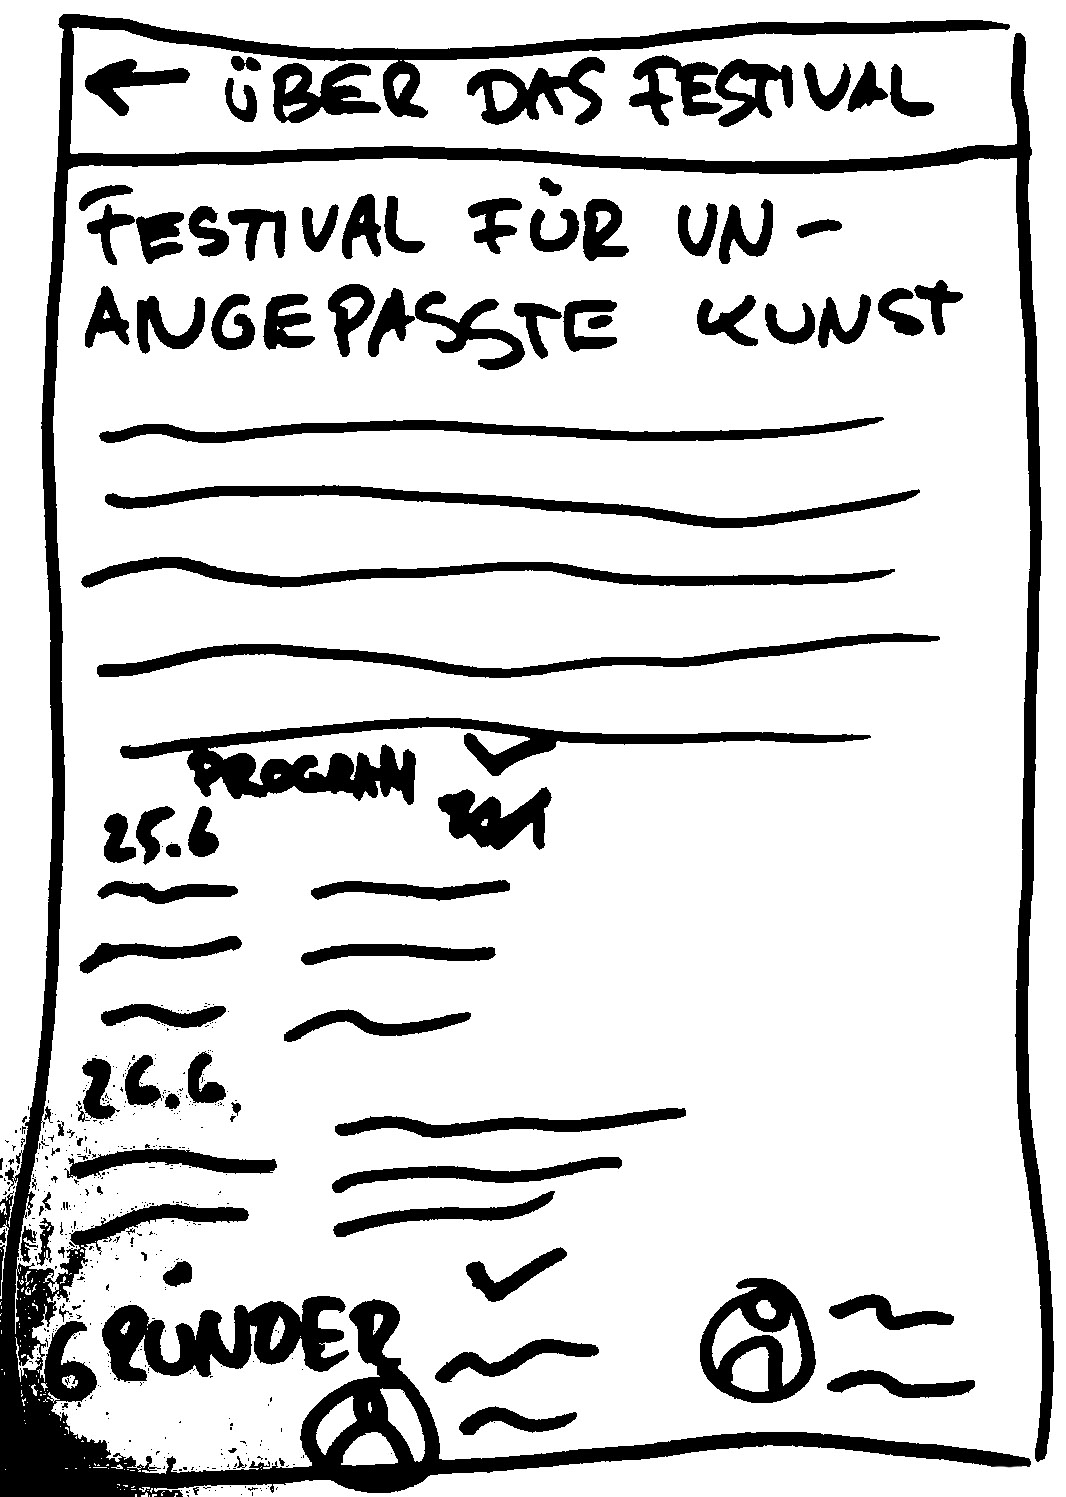
\includegraphics[width=\textwidth]{figures/festival-infos.jpg}
        \caption{Festival Informationen}
        \label{fig:gull}
    \end{subfigure}
    \begin{subfigure}[b]{0.22\textwidth}
        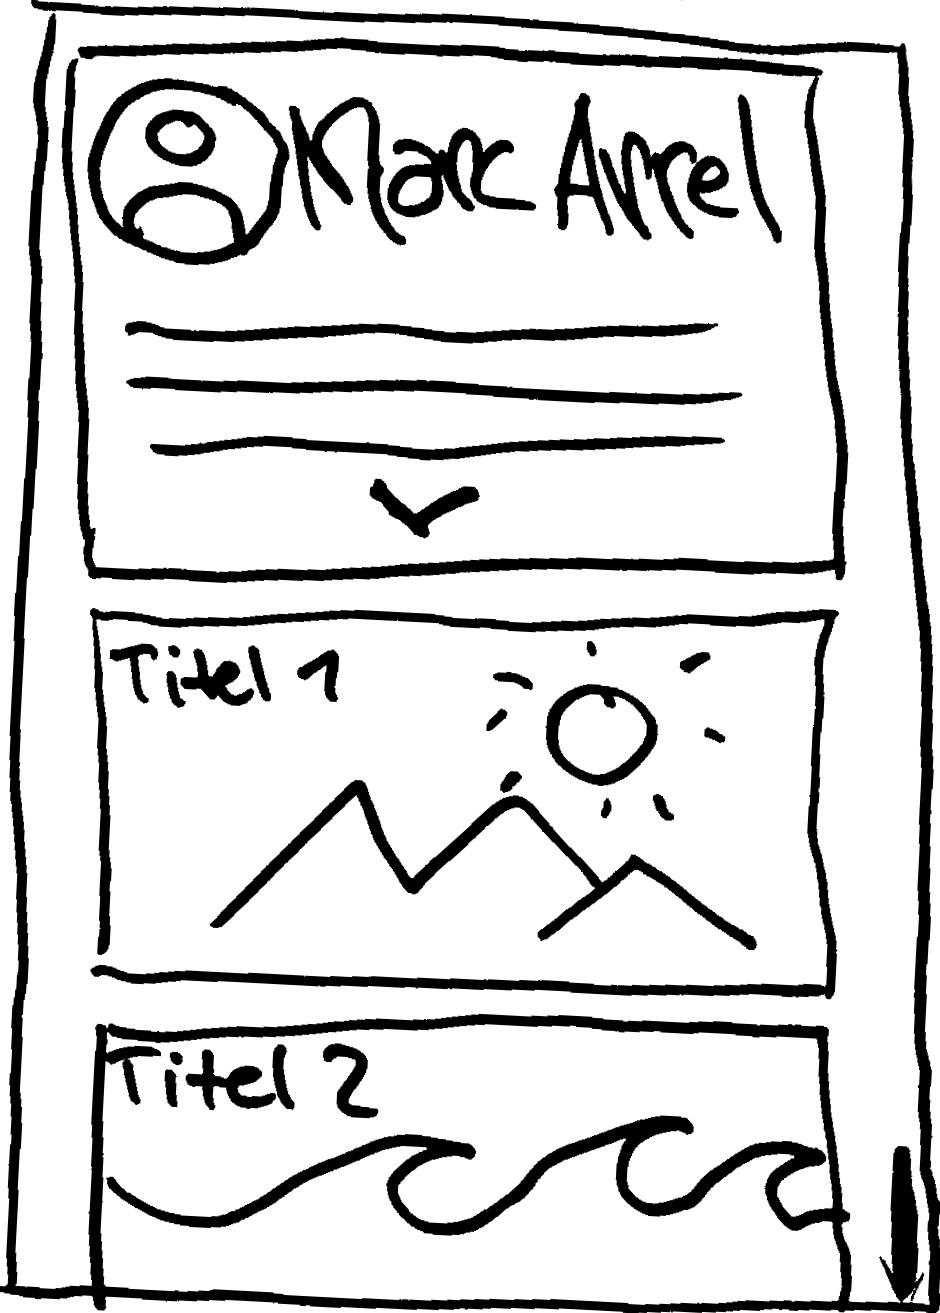
\includegraphics[width=\textwidth]{figures/kuenstler.jpg}
        \caption{Künstler Ansicht}
        \label{fig:tiger}
    \end{subfigure}
    \caption{Zwei erste Skizzen}
    \label{fig:skizzen}
\end{figure}
\subsection{Klick-Prototyp}
Mit den Einsichten aus den Skizzen und dem Paper Prototype haben wir einen \textit{high-fidelity} Klick-Prototyp erstellt. Dazu wurden Wireframes von allen Ansichten in Adobe Photoshop oder Adobe Illustrator erstellt. Diese wurden dann in Invision\footnote{\url{https://www.invisionapp.com/}} hochgeladen. Hier können die einzelnen Ansichten verknüpft und animiert werden. So entsteht ein Prototyp, der der finalen  App sehr ähnlich ist und der über einen Link von allen Teammitglieder aufgerufen, getestet und kommentiert werden kann (siehe Abbildung \ref{fig:prototype_werke}). Dadurch konnten wir weitere Schwächen und Unzulänglichkeiten der Gestaltung erkennen und ausbessern.

\begin{figure}[ht]
    \centering
        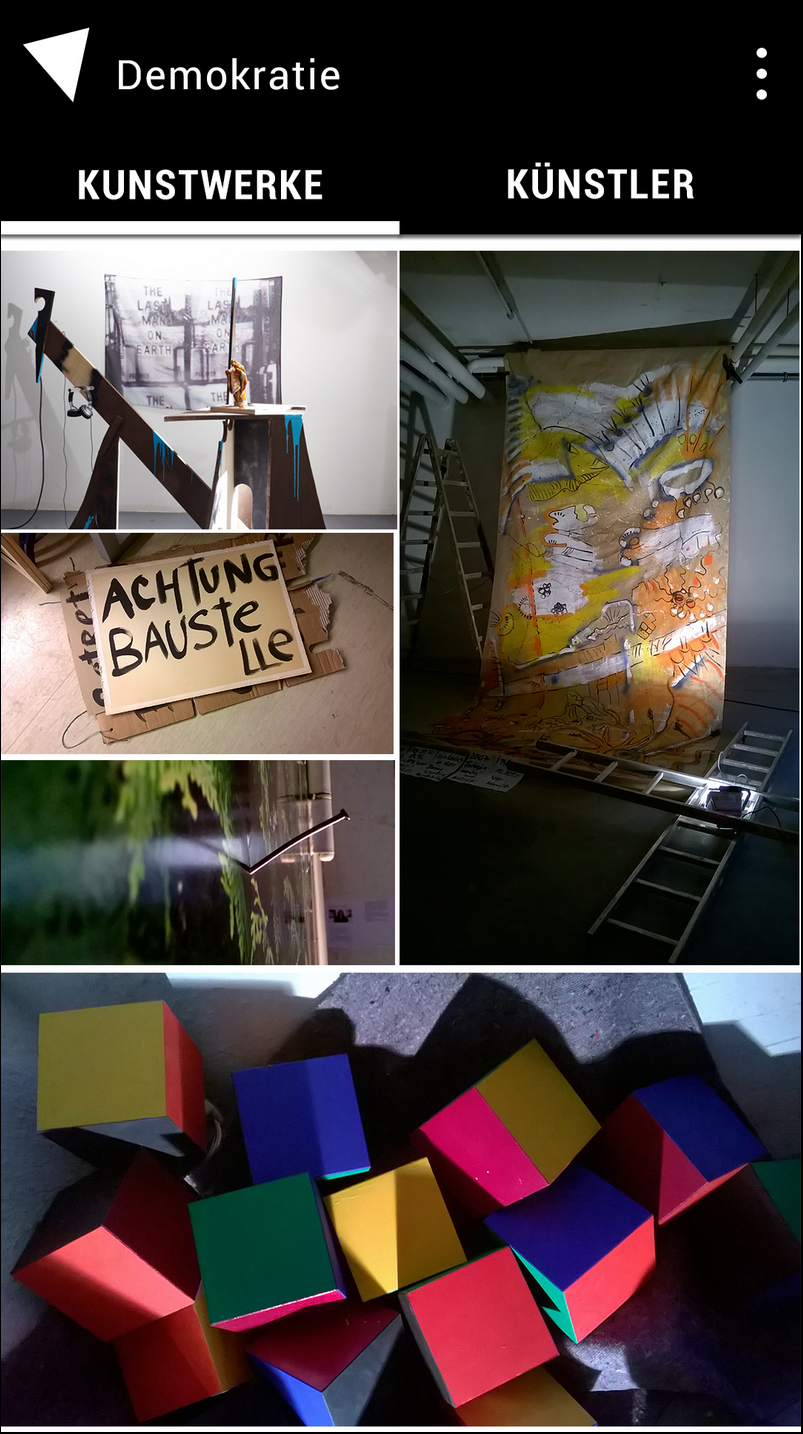
\includegraphics[width=.25\textwidth]{figures/prototype_werke.png}
    \caption{Übersicht der Werke des Klick-Prototypen}
    \label{fig:prototype_werke}
\end{figure}

\subsection{Entwicklung}
Zuletzt haben wir die Anwendung in Android implementiert. Als Entwicklungsumgebung wurde Android Studio verwendet, die Versionskontrolle erfolgte in Git. Natürlicherweise haben wir auch noch während der Entwicklung sowohl konzeptionelle als auch technische Probleme im Design gefunden, die ausgebessert werden mussten.